%!tex root = ../main.tex

\section{Results} \label{sec:results}

\lstset{
  basicstyle=\ttfamily,
  mathescape,
  columns=fixed,
  fontadjust=true,
  basewidth=0.5em
}

%\begin{figure}[H]
% \centering
% \includegraphics[]{example-image-duck}
% \caption{\todo{Illustration of k-lift using Theorem \ref{lem:lcl_unsolvability:from_klift_to_simple}}}
% \label{fig:duck2}
%\end{figure}

In this section, we will discuss the results from our implementation.
We answer to Research question~\ref{research_question:3} in Section~\ref{sec:results:improving_bounds} by finding new non-constant lower bounds for LCL problems that have already been classified with constant lower bounds prior this work.
In Section~\ref{sec:results:classifying_large_classes}, we answer to Research question~\ref{research_question:4} by finding new lower bounds for classes of LCL problems.
We use the implementation~\cite[commit \codee{c244e8e683}]{NonconstantLclClassifier2022} in its current state as of the time of writing this thesis.
When we say \codee{bin}, we refer to the compiled binary of the implementation.
Throughout this section, we assume that the results are obtained in a modern computer with AMD Ryzen 9 3900X 12-core 24-thread CPU, and 32 GB of RAM.

We do not use the caching feature of our implementation, as fetching already generated problem classes and multigraphs from the disk is substantially faster than generating them.
We want to give the measurements without pre-generated data unless we target some specific problems, like in Section~\ref{sec:results:improving_bounds}.

Earlier in Section~\ref{sec:lcl_problems:biregular}, we used the following notation to present the sets $A$ and $P$ of maximal independent set.
\begin{align*}
    %\Sigma &= \mathrm{\{I,O,P\}}, \\
    A &= \mathrm{\{\{I,I,I\},\{P,O,O\}\}}, \\
    P &= \mathrm{\{\{I,P\},\{I,O\},\{O,O\}\}}.
  \end{align*}
In the following sections, all LCL problems are presented in an alternative format, where each label in a label configuration are concatenated, and each label configuration is separated by a space.
Maximal independent set would be encoded as
$A = \text{III POO}$ and $P = \text{IP IO OO}$.
The problems are also normalized, as explained in Section~\ref{sec:implementation:generating_lcl_problems}.
Therefore, the problem is actually encoded as $A = \text{AAA BBC}$ and $P = \text{AB AC BB}$.


%We will answer to Research questions 3 by using our implementation for various LCL problems and showing their
%
%and 4 by showing classifications
%
\subsection{Improving Lower Bounds of LCL Problems}\label{sec:results:improving_bounds}
As we discussed in Section~\ref{sec:research_question}, we will be using a database~\cite{Tereshchenko2021,LclClassifierAalto,LclClassifierGithub} that consists of LCL problems and their current known lower and upper bounds.
There are two LCL problem classes in the database that are for non-directed non-rooted trees---$(\Delta, \delta, \lambda) = (3,2,3)$ and $(\Delta, \delta, \lambda) = (3,2,2)$.
All 38 problems of the class $(3,2,2)$ are already classified with tight deterministic bounds.
This is not the case in class $(3,2,3)$, therefore we try to find new deterministic lower bounds for the problems using our implementation.

We use the latest database dump~\cite{DatabaseDump} of the database.
In the class $(3,2,3)$, there are 7735 unique LCL-problems after purging and normalizing the problems, as we can see from Table~\ref{tbl:lcl_problem_classes}.
The database also agrees with the number of problems.

We are interested in the problems that have a constant ($\mathcal{O}(1)$) deterministic lower bound and a non-constant upper-bound, as these are the only problems for which we can possibly find a better lower bound of non-constant i.e.\ $\Omega(\log^*n)$.
When we remove problems with non-constant deterministic lower bounds, we get 6538 problems with a constant deterministic lower bound.
Out of these problems, we need to remove problems with constant upper bound, as these problems already have a tight constant bound, i.e.\ $\Theta(1)$.
After the removal, we have only 66 problems left.
The problems can be fetched from the database to a file \codee{problems.txt} using the command \verb|bin fetch_problems 3 2 3 <database_address> > problems.txt|, assuming that there is a PostgreSQL database in the address \verb|<database_address>| with the data from the dump.

% \begin{figure}[H]
% \centering
% \includegraphics[]{example-image-duck}
% \caption{\todo{Maybe add a figure that explains the upper and lower bounds we want the problems to have. }}
% \label{fig:duck2}
% \end{figure}

We execute our implementation using the command
\begin{lstlisting}
bin find <$\text{n}_{\text{low}}$> <$\text{n}_{\text{high}}$> --stats from_stdin < problems.txt
\end{lstlisting}
where $n_\text{low}$ and $n_\text{high}$ are substituted with smallest and highest number of vertices we want for the graphs, respectively.
The option \lstinline{--stats} gives us the execution times from generating graphs, and encoding/solving SAT problems.
We run the command as follows in Table~\ref{tbl:results:asd1}.

\begin{table}[H]
    \centering
    %\begin{adjustbox}{width={\textwidth},keepaspectratio}%
    \begin{tabular}{rrrrr}
        \toprule
        &&& \multicolumn{2}{c}{Time (s)} \\
        \cmidrule{4-5}
        $n_\text{low}$ & $n_\text{high}$ & \# of new lower bounds & Generate graphs & SAT\\
        \midrule
        %&&&&& \multicolumn{2}{c}{Trees} \\
        %Classifier & Complete & Labels & Paths & Cycles &Rooted & Unrooted \\\midrule
        1  & 5  & 1 & 0.031 & 0.002\\
        6  & 10 & 7 & 0.030 & 0.004\\
        11 & 15 & 8 & 0.062 & 0.015\\
        16 & 20 & 7 & 0.140 & 0.080\\
        21 & 25 & 7 & 3.758 & 0.510\\
        26 & 30 & 7 & 137.5\phantom{00} & 3.980\\
        %\vdots & \vdots &\vdots&\vdots\\
        \bottomrule
    \end{tabular}
    %\end{adjustbox}
    \caption{%
    Executing the command multiple times with different vertex ranges gives us new lower bounds.
    We can also see how long it takes to generate multigraphs, and also how long it takes to encode and solve SAT problems.
    }
    \label{tbl:results:asd1}
\end{table}

The executions from Table~\ref{tbl:results:asd1} were all executed with an identical input problem set, therefore some problems can be as a result in multiple executions.
When we consider only the smallest graph, where the problem was found to be unsolvable, there are only 9 distinct problems left.
The problems are listed in Table~\ref{tbl:results:asd2}.

\begin{table}[H]
    \centering
    \begin{adjustbox}{width={\textwidth},keepaspectratio}%
    \begin{tabular}{rlllllll}
        \toprule
        &&& \multicolumn{2}{c}{Lower bound} \\
        \cmidrule{4-5}
        $n$ & $A$ & $P$ & Old & New & Upper bound\\
        \midrule
        %&&&&& \multicolumn{2}{c}{Trees} \\
        %Classifier & Complete & Labels & Paths & Cycles &Rooted & Unrooted \\\midrule
        5  & AAA AAB BBC BCC     & AB CC       & $\Omega(1)$ & $\Omega(\log^*n)$ & $\mathcal{O}(\log n)$\\
        10 & AAA AAB ABC BCC     & AC BB       & $\Omega(1)$ & $\Omega(\log^*n)$ & $\mathcal{O}(\log n)$\\
        10 & AAA AAB ABC BCC     & AC BB CC    & $\Omega(1)$ & $\Omega(\log^*n)$ & $\mathcal{O}(\log n)$\\
        10 & AAA AAB ABC BCC CCC & AC BB       & $\Omega(1)$ & $\Omega(\log^*n)$ & $\mathcal{O}(\log n)$\\
        10 & AAA AAB ABC CCC     & AC BB       & $\Omega(1)$ & $\Omega(\log^*n)$ & $\mathcal{O}(\log n)$\\
        10 & AAA AAB BCC         & AC BB CC    & $\Omega(1)$ & $\Omega(\log^*n)$ & $\mathcal{O}(\log n)$\\
        10 & AAA ABC BBC         & AB BB CC    & $\Omega(1)$ & $\Omega(\log^*n)$ & $\mathcal{O}(\log n)$\\
        10 & AAA BBC             & AB BB CC    & $\Omega(1)$ & $\Omega(\log^*n)$ & $\mathcal{O}(\log n)$\\
        15 & AAA BBC             & AB AC BB CC & $\Omega(1)$ & $\Omega(\log^*n)$ & $\mathcal{O}(\log^* n)$\\
        %\vdots & \vdots &\vdots&\vdots&\vdots&\vdots&\vdots\\
        \bottomrule
    \end{tabular}
    \end{adjustbox}
    \caption{%
    New lower bounds for LCL problems from the class $(3,2,3)$.
    Here, the column $n$ indicates the size of the smallest multigraph, in which the problem is unsolvable.
    The last column lists the current known upper bound from the database.
    }
    \label{tbl:results:asd2}
\end{table}
We make an observation that the last problem with a new lower bound in Table~\ref{tbl:results:asd2} has a matching upper bound.
Therefore, this problem has now a tight bound of $\Theta(log^* n)$.
Also, we make an observation that it is a relaxation of the maximal independent set i.e.\ the set $P$ has an additional label configuration CC.

Next, in Table~\ref{tbl:results:asd3}, we list all the multigraphs in which we found the problems to be unsolvable.

\begin{table}[H]
    \centering
    %\begin{adjustbox}{width={\textwidth},keepaspectratio}%
    \begin{tabular}{ll|r|r|r|r|r|r}
        \toprule
        && \multicolumn{6}{c}{$n$} \\
        \cmidrule{3-8}
        $A$ & $P$ & 5&10&15&20&25&30\\
        \midrule
        %&&&&& \multicolumn{2}{c}{Trees} \\
        %Classifier & Complete & Labels & Paths & Cycles &Rooted & Unrooted \\\midrule
        AAA AAB BBC BCC     & AB CC       & 1 &   &          &     &     &    \\
        AAA BBC             & AB AC BB CC &   &   & $9$      &     &     &    \\
        AAA AAB ABC BCC     & AC BB CC    &   & 1 & $5,9,12$ & $X$ & $Y$ & $Z$\\
        AAA AAB ABC BCC     & AC BB       &   & 1 & $5,9,12$ & $X$ & $Y$ & $Z$\\
        AAA AAB ABC BCC CCC & AC BB       &   & 1 & $5,9,12$ & $X$ & $Y$ & $Z$\\
        AAA AAB ABC CCC     & AC BB       &   & 1 & $5,9,12$ & $X$ & $Y$ & $Z$\\
        AAA AAB BCC         & AC BB CC    &   & 1 & $5,9,12$ & $X$ & $Y$ & $Z$\\
        AAA ABC BBC         & AB BB CC    &   & 1 & $5,9,12$ & $X$ & $Y$ & $Z$\\
        AAA BBC             & AB BB CC    &   & 1 & $5,9,12$ & $X$ & $Y$ & $Z$\\
        %\vdots & \vdots &\vdots&\vdots&\vdots&\vdots&\vdots\\
        \bottomrule
    \end{tabular}
    %\end{adjustbox}
    \caption{%
    List of multigraphs in which the problems are unsolvable.
    The multigraphs are listed as identifiers under each graph size $n$, and these identifiers are each specific to the size $n$.
    The identifiers under sizes $20$, $25$ and $30$ are too large to be shown in this table, thus we use sets $X,Y,Z$.
    The sizes of these sets are $|X|=12, |Y|=66$ and $|Z|=424$.
    }
    \label{tbl:results:asd3}
\end{table}

We visualize the multigraphs of sizes $n \in \{5,10,15\}$ from Table~\ref{tbl:results:asd3}.
These graphs can be seen in Figure~\ref{fig:results:graphs}.

\begin{figure}[H]
  \captionsetup{justification=centering}
    \subcaptionbox{
        $n=5,$ \\ \phantom{(a)}$id=1.$
      \label{fig:results:graphs:n5_1}
    }%
    [0.13\textwidth]
    {
      \centering
      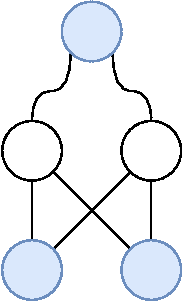
\includegraphics[scale=0.35]{diagrams/results_multigraph_n5_1.pdf}
    }
    \hfill
    \subcaptionbox{
      $n=10,$ \\ \phantom{(b)}$id=1.$
        %$n=10, id=1.$
      \label{fig:results:graphs:n10_1}
    }%
    %[0.20\textwidth]
       {
      \centering
      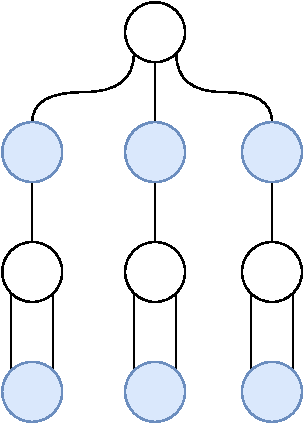
\includegraphics[scale=0.35]{diagrams/results_multigraph_n10_1.pdf}
    }
    \hfill
    \subcaptionbox{
      $n=15,$ \\ \phantom{(c)}$id=5.$
      \label{fig:results:graphs:n15_5}
    }%
       {
      \centering
      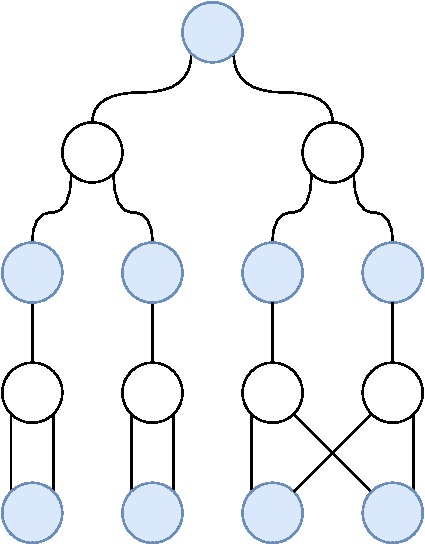
\includegraphics[scale=0.35]{diagrams/results_multigraph_n15_5.pdf}
    }
    \hfill
    \subcaptionbox{
      $n=15,$ \\ \phantom{(d)}$id=9.$
      \label{fig:results:graphs:n15_9}
    }%
       {
      \centering
      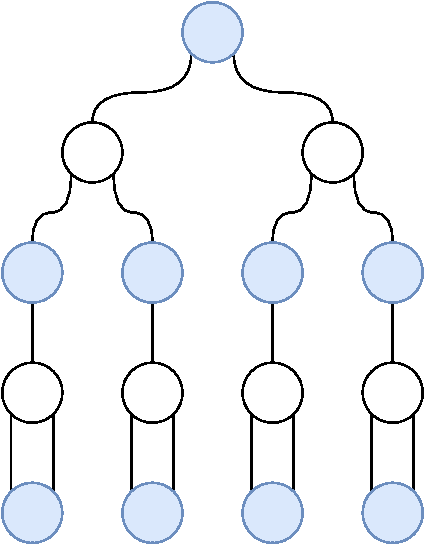
\includegraphics[scale=0.35]{diagrams/results_multigraph_n15_9.pdf}
    }
    \hfill
    \subcaptionbox{
      $n=15,$ \\ \phantom{(e)}$id=12.$
      \label{fig:results:graphs:n15_12}
    }%
       {
      \centering
      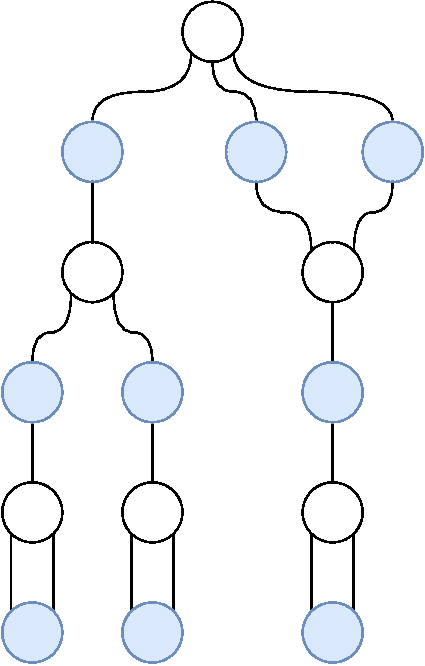
\includegraphics[scale=0.35]{diagrams/results_multigraph_n15_12.pdf}
    }
    \caption{All multigraphs from Table~\ref{tbl:results:asd3}, where $n \in \{5,10,15\}.$}
    \label{fig:results:graphs}
  \end{figure}


\subsection{Finding New Lower Bounds For Classes of LCL Problems} \label{sec:results:classifying_large_classes}
In this section, we try to find new lower bounds for various classes of LCL problems, with the focus on measuring performance.
We give the execution times of each execution similarly we did in Table~\ref{tbl:results:asd1}, except this time we exclude all problems with new lower bounds before executing the implementation with higher graph sizes.
We also use only the exact graph sizes that are possible with each problem class, as explained in Section~\ref{sec:implementation:generating_multigraphs}.
For example, there are only multigraphs of sizes $5, 10, 15, 20, 25, 30, ...$, with the problem class $(3,2,3)$.
In this section, we use a cache for problems, therefore only the first graph size for each example has the true generation time for problems, and all consequent entries in each table show the time it takes to fetch the problems from the cache.

Our first experiment with problem class $(7,5,2)$ is a failure, as seen in Table~\ref{tbl:results:new_lower_bounds_for_classes:7_5_2}.
We could not generate even the smallest multigraphs without the process being terminated.
The class has 7770 unique problems.
%For comparison, the class $(3,2,3)$ has 7735 problems.
At first, it seemed the class would be a good starting point, as previously in Section~\ref{sec:results:improving_bounds}, we ran the implementation with the class $(3,2,3)$, which has a similar number of problems (7735).
It seems that the degrees $\Delta=7$ and $\delta=5$ along with graph size $n=12$ results in too large set of graphs.
Our implementation cannot handle such cases, so there is a lot of room for improvements in the part of graph generation.
\begin{table}[H]
    \centering
    %\begin{adjustbox}{width={\textwidth},keepaspectratio}%
    \begin{tabular}{rrrrrr}
        \toprule
        && \multicolumn{3}{c}{Time (s)} \\
        \cmidrule{3-5}
        $n$ & \# of new lower bounds & Generate problems & Generate graphs & SAT\\
        \midrule
        %&&&&& \multicolumn{2}{c}{Trees} \\
        %Classifier & Complete & Labels & Paths & Cycles &Rooted & Unrooted \\\midrule
        12  & ?  & 0.068  & $>359$  & ?\\
        24 & ? & ? & ? & ? \\
        36 & ? & ? & ? & ? \\
        %\vdots & \vdots &\vdots&\vdots\\
        \bottomrule
    \end{tabular}
    %\end{adjustbox}
    \caption{%
    Failed experiment with the problem class $(7,5,2)$.
    The execution terminated early during generating graphs, probably because lack of memory.
    }
    \label{tbl:results:new_lower_bounds_for_classes:7_5_2}
\end{table}

Our second experiment is with problem class $(6,4,2)$.
We kept the label count same as in the first experiment, but we lower each degree by one.
Thus, there are only 1616 problems in the class.
The results can be seen in Table~\ref{tbl:results:new_lower_bounds_for_classes:6_4_2}.
This time we got new lower bounds at least for some problems.
\begin{table}[H]
    \centering
    %\begin{adjustbox}{width={\textwidth},keepaspectratio}%
    \begin{tabular}{rrrrrr}
        \toprule
        && \multicolumn{3}{c}{Time (s)} \\
        \cmidrule{3-5}
        $n$ & \# of new lower bounds & Generate problems & Generate graphs & SAT\\
        \midrule
        %&&&&& \multicolumn{2}{c}{Trees} \\
        %Classifier & Complete & Labels & Paths & Cycles &Rooted & Unrooted \\\midrule
        5  & 250  & 0.036  & 0.053  & 0.188\\
        10 & 21 & 0.002 & 0.373 & 47.5\phantom{00} \\
        15 & ? & $<1$\phantom{.000} & $>453$\phantom{.000} & ? \\
        %\vdots & \vdots &\vdots&\vdots\\
        \bottomrule
    \end{tabular}
    %\end{adjustbox}
    \caption{%
    New lower bounds for problems from the class $(6,4,2)$.
    The execution terminates at $n=15$ during the generation of graphs, probably for the same reason it terminated in the first experiment.
    }
    \label{tbl:results:new_lower_bounds_for_classes:6_4_2}
\end{table}

In Research question~\ref{research_question:4}, we ask if we can make the implementation fast enough to classify large classes of problems.
The class $(7,5,2)$ with size 7770 was definitely too large for our implementation, because of the high degrees.
The class $(3,2,3)$ has roughly the same size (7735) and it could be classified using graphs up to size $n=30$.
On the other hand the class $(6,4,2)$ had only 1616 problems, but we were able to classify the problems using graphs up to size $n=10$.
It seems that the answer depends a lot on the definition of what is a large class of problems.
In this thesis, we consider a problem class with over 1000 problems as large.
With this definition, we get an answer of yes, with some classes.

The bottleneck that causes our implementation to terminate early is the graph generation.
We make an observation that the large classes that can be classified fast are the classes with low number of degrees, because then there is only a low number of graphs, thus no running out of memory.
